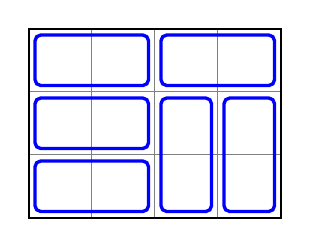
\begin{tikzpicture}[scale=0.8]
  % grid of a 4 x 3 board
  \draw[gray] (0,0) grid (4,3);
  % dominoes: three horizontal on the left, one horizontal top right, two vertical bottom right
  \foreach \y in {0,1,2} {
    \draw[blue, very thick, rounded corners=2pt] (0.1,\y+0.1) rectangle (1.9,\y+0.9);
  }
  \draw[blue, very thick, rounded corners=2pt] (2.1,2.1) rectangle (3.9,2.9);
  \draw[blue, very thick, rounded corners=2pt] (2.1,0.1) rectangle (2.9,1.9);
  \draw[blue, very thick, rounded corners=2pt] (3.1,0.1) rectangle (3.9,1.9);
  \draw[thick] (0,0) rectangle (4,3);
\end{tikzpicture}
